\chapter{Implementacja sprzętowa}

\section{Binaryzacja}

W celu ekstrakcji obrazu zbinaryzowanego z~obrazu w~formacie RGB zdecydowano się wykorzystać binaryzację ze stałym progiem. 
Obraz wejściowy najpierw konwertowany jest do obrazu w~odcieniach szarości. 
W~formacie RGB na każdy piksel składają się trzy kanały, każdy o~wartości z~przedziału 0-255 zapisane na 8 bitach. 
Największe i najmniejsze wartości z~kanałów są dodawane i~dzielone przez 2. 
Operacja ta zostaje przeprowadzona dla każdego piksela.
Zdecydowano się na taką metodę, ponieważ dzielenie przez liczbę, która jest wielokrotnością 2 może zostać zrealizowane poprzez przesunięcie bitowe. Jest ono znacznie szybsze niż użycie dzielarki. W porównaniu do wyliczania średniej z trzech kanałów, zachowujemy pełny zakres od 0 do 255 i nie musimy wykorzystywać dzielarki.
Obrazem wynikowym jest obraz w~odcieniach szarości, który kolejno jest poddawany binaryzacji.

\noindent Rysunki \ref{fig:in_otsu_fpga}, \ref{fig:out_otsu_fpga} przedstawiają efekt symulacji tego algorytmu dla obrazu o~wymiarach 348x128. 

\begin{figure}[h]
		\centering
		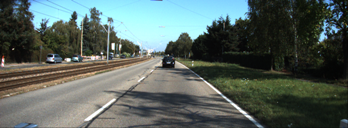
\includegraphics[scale=0.8]{obraz_color_smal.png}
		\caption{Obraz wejściowy do symulacji sprzętowej binaryzacji}
		\label{fig:in_otsu_fpga}
\end{figure}

\begin{figure}[h]
		\centering
		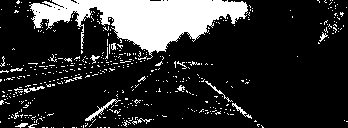
\includegraphics[scale=0.8]{obraz_bin_smal.png}
		\caption{Obraz wyjściowy z symulacji sprzętowej binaryzacji}
		\label{fig:out_otsu_fpga}
\end{figure}

\section{Wyznaczanie ROI}
Efekty symulacji implementacji sprzętowej wyznaczania obszaru zainteresowania zostały przedstawione na rysunku \ref{fig:roi_sym}.


Opis schematu \ref{fig:roi_symmm} implementacji sprzętowej algorytmu do wyznaczenia współczynników wykorzystywanych w \ref{fig:roi_symm2}(w nawiasach podano liczbę bitów potrzebną do zapisania danej wartości albo liczbę taktów zegara potrzebnych do przeprowadzania danej operacji):
\begin{itemize}
	\item A - współrzędna x piksela, poz\_x (12 bity),
	\item B - stała wartość równa 3 (4 bity),
	\item C - jedna ósma szerokości obrazu (12 bitów),
	\item D - stała wartość równa 5 (4 bity),
	\item W1 - współczynnik 1 (16 bitów),
	\item W2 - współczynnik 2 (16 bitów),
	\item (-) - odejmowanie (1 takt zegara),
\end{itemize}
Rezultaty odejmowania W1 i W2 są kolejno wykorzystywane w logice asynchronicznej \ref{fig:roi_symm2}
\begin{figure}[h]
	\centering
	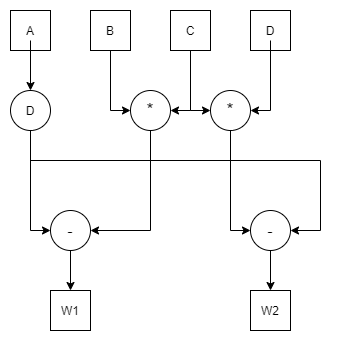
\includegraphics[scale=0.5]{ROI_schem.png}
	\caption{Schemat algorytmu do wyznaczania współczynników dla ROI.}
	\label{fig:roi_symmm}
\end{figure}
\begin{figure}[h]
	\centering
	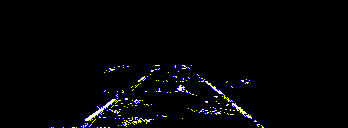
\includegraphics[scale=0.8]{obraz_roi_smal.png}
	\caption{Obraz wyjściowy z symulacji sprzętowej algorytmu do wyznaczania ROI.}
	\label{fig:roi_sym}
\end{figure}

\begin{figure}[h]
	\centering
	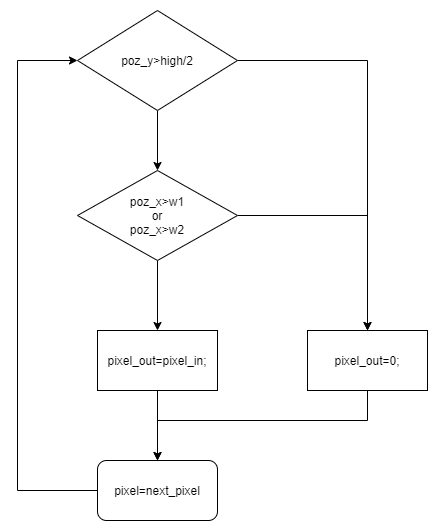
\includegraphics[scale=0.5]{ROI_blockowy.png}
	\caption{Schemat algorytmu do wyznaczania ROI. Wartości współczynnik1 i współczynnik2 są rezultatami \ref{fig:roi_symmm}}
	\label{fig:roi_symm2}
\end{figure}
\section{LMPS}

\begin{figure}[h]
	\centering
	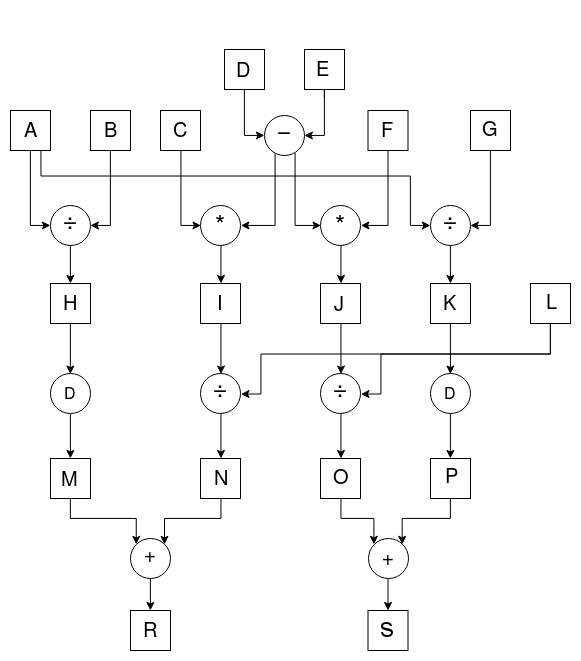
\includegraphics[scale=0.4]{impl_dev_lmps_1.png}
	\caption{Schemat blokowy implementacji sprzętowej algorytmu do wyznaczenia ograniczeń górnych i dolnych dla filtru LMPS}
	\label{fig:lmps1}
\end{figure}

Opis schematu implementacji sprzętowej algorytmu do wyznaczenia ograniczeń górnych i~dolnych \ref{fig:lmps1}:
\begin{itemize}
	\item A - szerokość obrazu (32 bity),
	\item B - stała zależna od grubości linii drogowych, wynosi 400 (20 bitów),
	\item C - stała zależna od grubości linii drogowych, wynosi 20 (8 bitów),
	\item D - indeks wiersza obecnego piksela (24 bity),
	\item E - połowa szerokości obrazu (24 bity),
	\item F - stała zależna od grubości linii drogowych, wynosi 62 (8bitów),
	\item G - stała zależna od grubości linii drogowych, wynosi 90 (20 bitów),
	\item L - wysokość obrazu (20 bitów),
	\item H, K, N, O - rezultaty dzielenia (32 bity),
	\item I, J - rezultaty mnożenia (32 bity),
	\item M, P - sygnały wyjściowe z linii opóźniających (32 bity),
	\item R - próg ograniczający dolny (32 bity),
	\item S - próg ograniczający górny (32 bity),
	\item ($\div$) - dzielenie (4 takty zegara),
	\item (*) - mnożenie (1 takt zegara),
	\item (D) - linia opóźniająca (1 takt zegara),
	\item (+) - dodawanie (1 takt zegara).
	\item (-) - odejmowanie (1 takt zegara).
\end{itemize}
Progi ograniczające dolny i~górny wykorzystywane są kolejno w~logice asynchronicznej przedstawionej na schemacie \ref{fig:lmps2}. 
Nie zamieszczono rysunków z~symulacji implementacji sprzętowej, ponieważ dla obrazów o~rozmiarze tak małym jak 348x128, filtr nie daje rzetelnych rezultatów. 
W~modelu programowym wykorzystano obraz o~rozmiarze 1392x512. 
Tak znaczne zmniejszenie go oraz zniekształcenie powoduje zaburzenie działania filtru. 
Wynika to z~tego, że działanie filtru jest zależne od wysokości i~szerokości obrazu.

\begin{figure}[!]
	\centering
	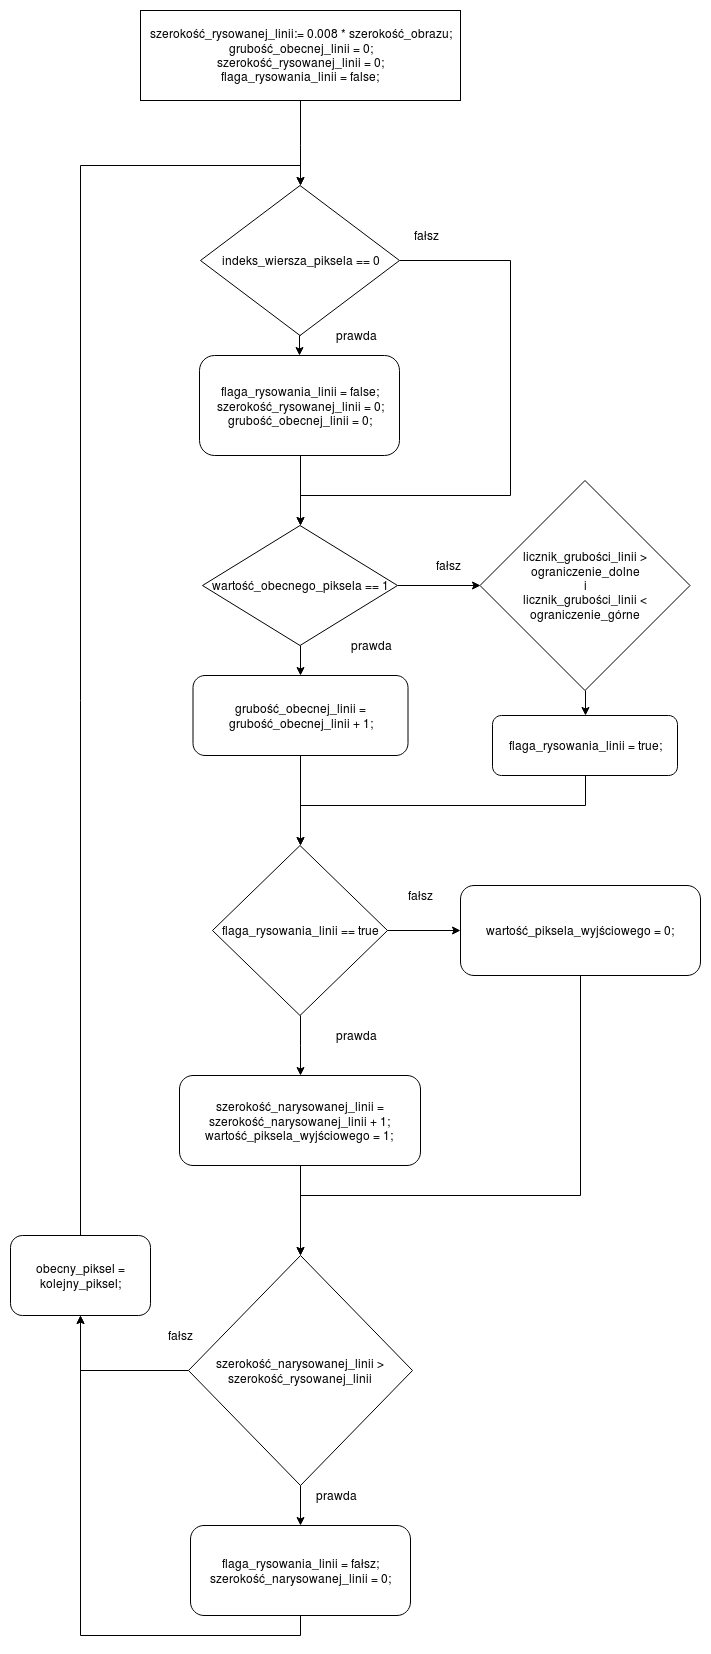
\includegraphics[scale=0.35]{impl_dev_lmps_2.png}
	\caption{Schemat blokowy implementacji sprzętowej algorytmu do odfiltrowania elementów nie będących liniami ruchu drogowego.}
	\label{fig:lmps2}
\end{figure}


\section{Podział obrazu}

W celu wyznaczenia środków ciężkości w określonych strefach na obrazie, wykorzystuje się implementacje sprzętową(dla każdego obszaru oddzielnie) przedstawioną na schemacie \ref{fig:wyzn_sc}. Jeśli, któryś z liczników po przeiterowaniu całego obrazu jest równy 0, środek nie jest wyznaczany.
\begin{figure}[h]
	\centering
	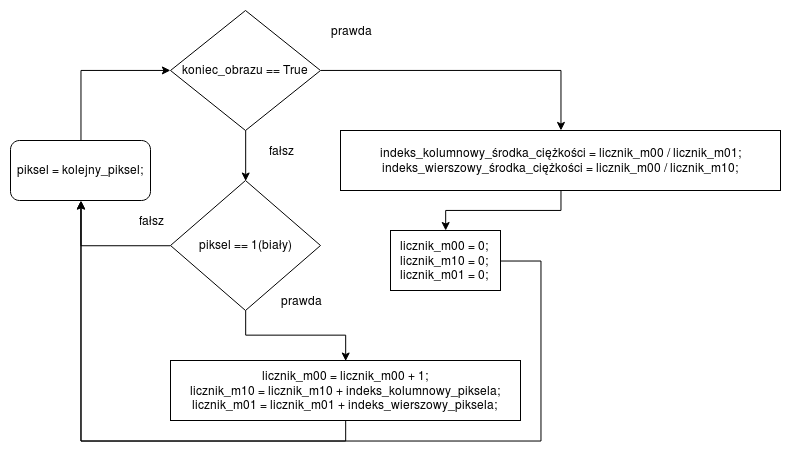
\includegraphics[scale=0.6]{wyzn_sc.png}
	\caption{Schemat blokowy implementacji sprzętowej algorytmu do wyznaczenia środka ciężkości.}
	\label{fig:wyzn_sc}
\end{figure}